% Figure 5.1. Full design domain and its left-half symmetry-reduced domain (side by side).
% Labels use \normalsize; the figure is included at \textwidth (150 mm) with scale ~0.93.
% Build in WSL: latex + dvips -E for EPS, pdflatex for PDF, pdftocairo for PNG.
\documentclass[tikz,border=3pt]{standalone}
\usepackage{amsmath}
\usepackage{tikz}
\usetikzlibrary{arrows.meta}

\begin{document}
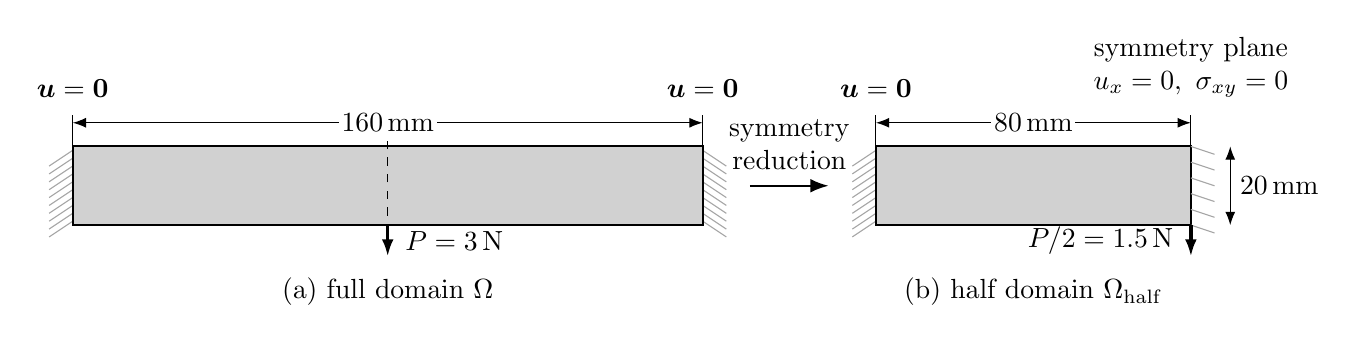
\begin{tikzpicture}[x=0.05cm,y=0.05cm,>=Latex,font=\normalsize]
  \def\L{160}
  \def\H{20}
  \def\Lhalf{80}
  \def\Xhalf{204}  % 左半域左端横坐标, 与完整域右端留 44 单位间隙

  % ================= 完整设计域 (左) =================
  \draw[thick,fill=black!18] (0,0) rectangle (\L,\H);
  \foreach \y in {0,2,...,18} {
    \draw[gray!70] (-6,\y-3) -- (0,\y+1);
    \draw[gray!70] (\L+6,\y-3) -- (\L,\y+1);
  }
  \draw[thick] (0,0) -- (0,\H);
  \draw[thick] (\L,0) -- (\L,\H);
  \draw[dashed] (0.5*\L,-6) -- (0.5*\L,\H+2);

  % 长度标注
  \draw[thin] (0,\H) -- (0,\H+8);
  \draw[thin] (\L,\H) -- (\L,\H+8);
  \draw[<->,thin] (0,\H+6) -- (\L,\H+6)
    node[midway,fill=white,inner sep=1pt] {$160\,\mathrm{mm}$};

  % 固支端标注 (单行)
  \node[anchor=south] at (0,\H+10) {$\boldsymbol{u}=\boldsymbol{0}$};
  \node[anchor=south] at (\L,\H+10) {$\boldsymbol{u}=\boldsymbol{0}$};

  % 中点载荷
  \draw[very thick,-{Latex[length=2.2mm,width=1.5mm]}] (0.5*\L,0) -- (0.5*\L,-8);
  \node[anchor=west] at (0.5*\L+2,-4) {$P=3\,\mathrm{N}$};
  \node at (0.5*\L,-17) {(a) full domain $\Omega$};

  % ============ 对称降维箭头 (两行标注) ============
  \draw[->,thick] (\L+12,0.5*\H) -- (\Xhalf-12,0.5*\H)
    node[midway,above=2pt,align=center] {symmetry\\reduction};

  % ================= 左半计算域 (右) =================
  \draw[thick,fill=black!18] (\Xhalf,0) rectangle (\Xhalf+\Lhalf,\H);
  \foreach \y in {0,2,...,18} {
    \draw[gray!70] (\Xhalf-6,\y-3) -- (\Xhalf,\y+1);
  }
  \draw[thick] (\Xhalf,0) -- (\Xhalf,\H);
  \draw[thick] (\Xhalf+\Lhalf,0) -- (\Xhalf+\Lhalf,\H);
  \foreach \y in {0,4,...,20} {
    \draw[gray!70] (\Xhalf+\Lhalf,\y) -- (\Xhalf+\Lhalf+6,\y-2);
  }

  % 尺寸标注
  \draw[thin] (\Xhalf,\H) -- (\Xhalf,\H+8);
  \draw[thin] (\Xhalf+\Lhalf,\H) -- (\Xhalf+\Lhalf,\H+8);
  \draw[<->,thin] (\Xhalf,\H+6) -- (\Xhalf+\Lhalf,\H+6)
    node[midway,fill=white,inner sep=1pt] {$80\,\mathrm{mm}$};
  \draw[<->,thin] (\Xhalf+\Lhalf+10,0) -- (\Xhalf+\Lhalf+10,\H)
    node[midway,right] {$20\,\mathrm{mm}$};

  % 边界条件标注
  \node[anchor=south] at (\Xhalf,\H+10) {$\boldsymbol{u}=\boldsymbol{0}$};
  \node[align=center,anchor=south] at (\Xhalf+\Lhalf,\H+10)
    {symmetry plane\\$u_x=0,\ \sigma_{xy}=0$};

  % 对称面底端载荷 (标注置于箭头左侧)
  \draw[very thick,-{Latex[length=2.2mm,width=1.5mm]}] (\Xhalf+\Lhalf,0) -- (\Xhalf+\Lhalf,-8);
  \node[anchor=east] at (\Xhalf+\Lhalf-2,-4) {$P/2=1.5\,\mathrm{N}$};
  \node at (\Xhalf+0.5*\Lhalf,-17) {(b) half domain $\Omega_{\mathrm{half}}$};
\end{tikzpicture}
\end{document}
